\documentclass[border=2pt]{standalone}
\usepackage[dvipsnames,svgnames,x11names]{xcolor}
\usepackage{tikz,amsmath,amssymb,bm}
\usetikzlibrary{backgrounds, calc, positioning}
\usetikzlibrary{arrows, decorations.pathmorphing, arrows.meta}
\usetikzlibrary{braids}
\pagestyle{empty}

% pdftoppm can convert pdf -> png
\begin{document}

%% Fig 1
\begin{tikzpicture}
\def\rowsep{1.8}
\def\labelx{-1.2} 
\def\labely{0.5}
\def\labeldist{0pt}


\node (B11) at (0,0) {
    \begin{tikzpicture}
    \pic [rotate=90, braid/.cd,
        width=15pt,
        number of strands=3,
        every strand/.style={ultra thick},
        strand 1/.style={Firebrick2},
        strand 2/.style={SeaGreen},
        strand 3/.style={Blue3},
    ] {braid={s_1 s_2}};
    \end{tikzpicture}
};

\node (B12) at (4,0) {
    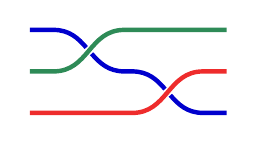
\begin{tikzpicture}
    \pic [rotate=90, braid/.cd,
        width=15pt,
        number of strands=3,
        every strand/.style={ultra thick},
        strand 1/.style={Firebrick2},
        strand 2/.style={SeaGreen},
        strand 3/.style={Blue3},
    ] {braid={s_2 s_1}};
    \end{tikzpicture}
};

\node at ($(B11.east)!0.5!(B12.west)$) {\Large $\neq$};
\node[below=\labeldist of B11] {$\sigma_1\sigma_2$};
\node[below=\labeldist of B12] {$\sigma_2\sigma_1$};

\node (B21) at (0,-\rowsep)  {
    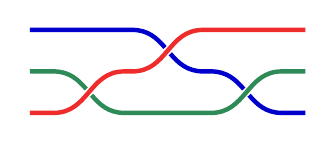
\begin{tikzpicture}
    \pic [rotate=90, braid/.cd,
        width=15pt,
        number of strands=3,
        every strand/.style={ultra thick},
        strand 1/.style={Firebrick2},
        strand 2/.style={SeaGreen},
        strand 3/.style={Blue3},
    ] {braid={s_1 s_2 s_1}};
    \end{tikzpicture}
};

\node (B22) at (4,-\rowsep) {
    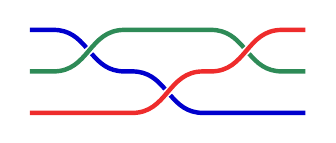
\begin{tikzpicture}
    \pic [rotate=90, braid/.cd,
        width=15pt,
        number of strands=3,
        every strand/.style={ultra thick},
        strand 1/.style={Firebrick2},
        strand 2/.style={SeaGreen},
        strand 3/.style={Blue3},
    ] {braid={s_2 s_1 s_2}};
    \end{tikzpicture}
};

\node at ($(B21.east)!0.5!(B22.west)$) {\Large $\equiv$};
\node[below=\labeldist of B21] {$\sigma_1\sigma_2\sigma_1$};
\node[below=\labeldist of B22] {$\sigma_2\sigma_1\sigma_2$};


\node (B31) at (0,-2*\rowsep) {
    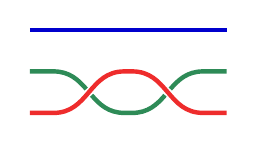
\begin{tikzpicture}
    \pic [rotate=90, braid/.cd,
        width=15pt,
        number of strands=3,
        every strand/.style={ultra thick},
        strand 1/.style={Firebrick2},
        strand 2/.style={SeaGreen},
        strand 3/.style={Blue3},
    ] {braid={s_1 s_1^{-1}}};
    \end{tikzpicture}
};

\node (B32) at (4,-2*\rowsep) {
    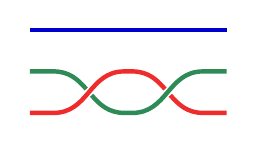
\begin{tikzpicture}
    \pic [rotate=90, braid/.cd,
        width=15pt,
        number of strands=3,
        every strand/.style={ultra thick},
        strand 1/.style={Firebrick2},
        strand 2/.style={SeaGreen},
        strand 3/.style={Blue3},
    ] {braid={s_1 s_1}};
    \end{tikzpicture}
};
\node[below=\labeldist of B31]{$\sigma_1\sigma_1^{-1} = I$};
\node[below=\labeldist of B32] {$(\sigma_1)^2 \neq I$};

\node[anchor=east,font=\bfseries] at (\labelx,\labely) {(A)}; \node[anchor=east,font=\bfseries] at (\labelx,{-\rowsep+\labely+0.28}) {(B)}; 
\node[anchor=east,font=\bfseries] at (\labelx,{-2*\rowsep+\labely}) {(C)};

\draw[->, thick] (0.0,1.0) -- (4.0,1.0) node[right] {time};

\end{tikzpicture}

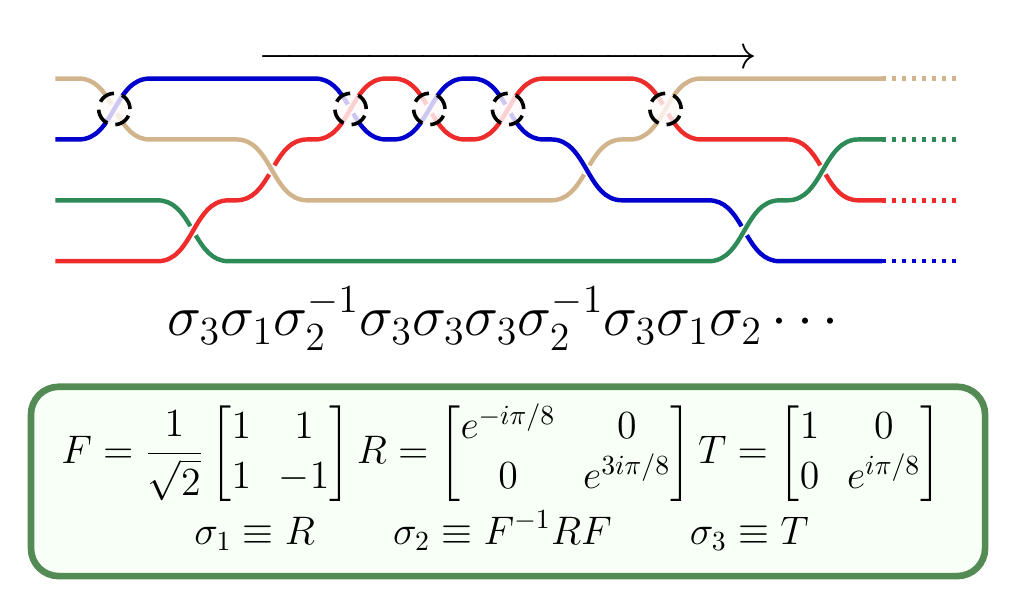
\begin{tikzpicture}

\begin{scope}[local bounding box=col1]
\pic (b) [
  rotate=90,
  braid/.cd,
  width=22pt,
  number of strands=4,
  every strand/.style={ultra thick},
  strand 1/.style={Firebrick2},
  strand 2/.style={SeaGreen},
  strand 3/.style={Blue3},
  strand 4/.style={Tan},
]
{braid={
s_3 s_1 s_2^{-1} s_3 s_3 s_3 s_2^{-1} s_3 s_1 s_2
}};

\tikzset{
  connection circle/.style={
    draw=black,
    thick, circle,
    fill=Snow,
    fill opacity=0.8,
    inner sep = 4pt,
    dash pattern=on 6pt off 3pt,
    line width = 1.3pt
  }
}


\foreach \level in {8} {
    \node [connection circle]
      at ($(b-1-\the\numexpr\level-1\relax)!0.5!(b-1-\level)$) {};
}

\foreach \level in {1,4,5,6} {
    \node [connection circle]
      at ($(b-3-\the\numexpr\level-1\relax)!0.5!(b-3-\level)$) {};
}

\draw[ultra thick, dotted, Firebrick2] (b-1-e) -- ++(1.0,0);
\draw[ultra thick, dotted, SeaGreen] (b-2-e) -- ++(1.0,0);
\draw[ultra thick, dotted, Blue3] (b-3-e) -- ++(1.0,0);
\draw[ultra thick, dotted, Tan] (b-4-e) -- ++(1.0,0);

\node[above] at (col1.north) {\LARGE $\xrightarrow{\hspace{6cm}}$};
\node[below=0.2cm] at (col1.south) {\huge $\sigma_3 \sigma_1 \sigma_2^{-1} \sigma_3 \sigma_3 \sigma_3 \sigma_2^{-1} \sigma_3 \sigma_1 \sigma_2\cdots$};
\node[below=0.3cm, draw=PaleGreen4, inner sep=6pt, align=center, fill=Honeydew1!50, rounded corners=10pt, line width=2.4pt] at (col1.south) {
\Large
$
\begin{array}{c}
\displaystyle
F = \frac{1}{\sqrt{2}}
\begin{bmatrix}
1 & 1\\
1 & -1
\end{bmatrix}
R =
\begin{bmatrix}
e^{-i\pi/8} & 0\\
0 & e^{3i\pi/8}
\end{bmatrix}
T =
\begin{bmatrix}
1 & 0\\
0 & e^{i\pi/8}
\end{bmatrix}
\\[0.8em]
\displaystyle
\sigma_1 \equiv R \qquad \sigma_2 \equiv F^{-1}RF \qquad \sigma_3 \equiv T
\end{array}
$
};
\end{scope}

\end{tikzpicture}

\par

\begin{tikzpicture}

\begin{scope}[local bounding box=col1]
\pic (b) [
  rotate=90,
  braid/.cd,
  width=22pt,
  number of strands=3,
  every strand/.style={ultra thick},
  strand 1/.style={Firebrick2},
  strand 2/.style={SeaGreen},
  strand 3/.style={Blue3},
  strand 4/.style={Tan},
]
{braid={
s_1^{-1} s_2 s_1 s_2^{-1} s_1 s_1 s_2^{-1} s_1 s_2^{-1} s_1
}};

\draw[ultra thick, dotted, Firebrick2]   (b-1-e) -- ++(1.0,0);
\draw[ultra thick, dotted, SeaGreen] (b-2-e) -- ++(1.0,0);
\draw[ultra thick, dotted, Blue3]  (b-3-e) -- ++(1.0,0);

\node[above] at (col1.north) {\LARGE $\xrightarrow{\hspace{6cm}}$};
\node[below=0.2cm] at (col1.south) {\huge $\sigma_1^{-1} \sigma_2 \sigma_1 \sigma_2^{-1} \sigma_1 \sigma_1 \sigma_2^{-1} \sigma_1 \sigma_2^{-1} \sigma_1\cdots$};

\node[below=0.2cm, draw=RoyalBlue4, inner sep=6pt, align=center, fill=RoyalBlue4!15, rounded corners=10pt, line width=2.4pt] at (col1.south) { \Large $F = \begin{bmatrix}
1/\phi & 1/\sqrt{\phi} \\
1/\sqrt{\phi} & -1/\phi
\end{bmatrix}
R = \begin{bmatrix}
e^{-\frac{4i\pi}{5}} & 0 \\
0 & e^{\frac{3i\pi}{5}}
\end{bmatrix}
\begin{aligned}
    &\phi = \frac{1+\sqrt{5}}{2}\\
    &\sigma_1 = R\\
    &\sigma_2 = F^{-1}R F
\end{aligned}$};

\node[below=0.3cm] at (col1.south) {\Large
    $\sigma_1\equiv$ \begin{tikzpicture}[baseline=(current bounding box.center)]
    \pic (b2) [
      rotate=90,
      braid/.cd,
      width=20pt,
      number of strands=3,
      every strand/.style={ultra thick},
      strand 1/.style={Firebrick2},
      strand 2/.style={SeaGreen},
      strand 3/.style={Blue3},
    ]
    {braid={s_1}};
    \end{tikzpicture}

    $\sigma_2\equiv$ 
\begin{tikzpicture}[baseline=(current bounding box.center)]
    \pic (b2) [
      rotate=90,
      braid/.cd,
      width=20pt,
      number of strands=3,
      every strand/.style={ultra thick},
      strand 1/.style={Firebrick2},
      strand 2/.style={SeaGreen},
      strand 3/.style={Blue3},
    ]
    {braid={s_2}};
    \end{tikzpicture}

    $\sigma_1^{-1}\equiv$ 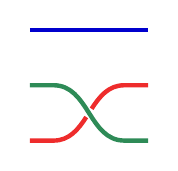
\begin{tikzpicture}[baseline=(current bounding box.center)]
    \pic (b2) [
      rotate=90,
      braid/.cd,
      width=20pt,
      number of strands=3,
      every strand/.style={ultra thick},
      strand 1/.style={Firebrick2},
      strand 2/.style={SeaGreen},
      strand 3/.style={Blue3},
    ]
    {braid={s_1^{-1}}};
    \end{tikzpicture}

    $\sigma_2^{-1}\equiv$ 
\begin{tikzpicture}[baseline=(current bounding box.center)]
    \pic (b2) [
      rotate=90,
      braid/.cd,
      width=20pt,
      number of strands=3,
      every strand/.style={ultra thick},
      strand 1/.style={Firebrick2},
      strand 2/.style={SeaGreen},
    strand 3/.style={Blue3},
    ]
    {braid={s_2^{-1}}};
    \end{tikzpicture}
};

\end{scope}

\end{tikzpicture}


\end{document}
